\sectionframe{Grundlegende Datentypen und Operatoren}
\begin{frame}
 \frametitle{Aufbau einer einfachen Zuweisungsanweisung}
 \begin{figure}
  \centering
  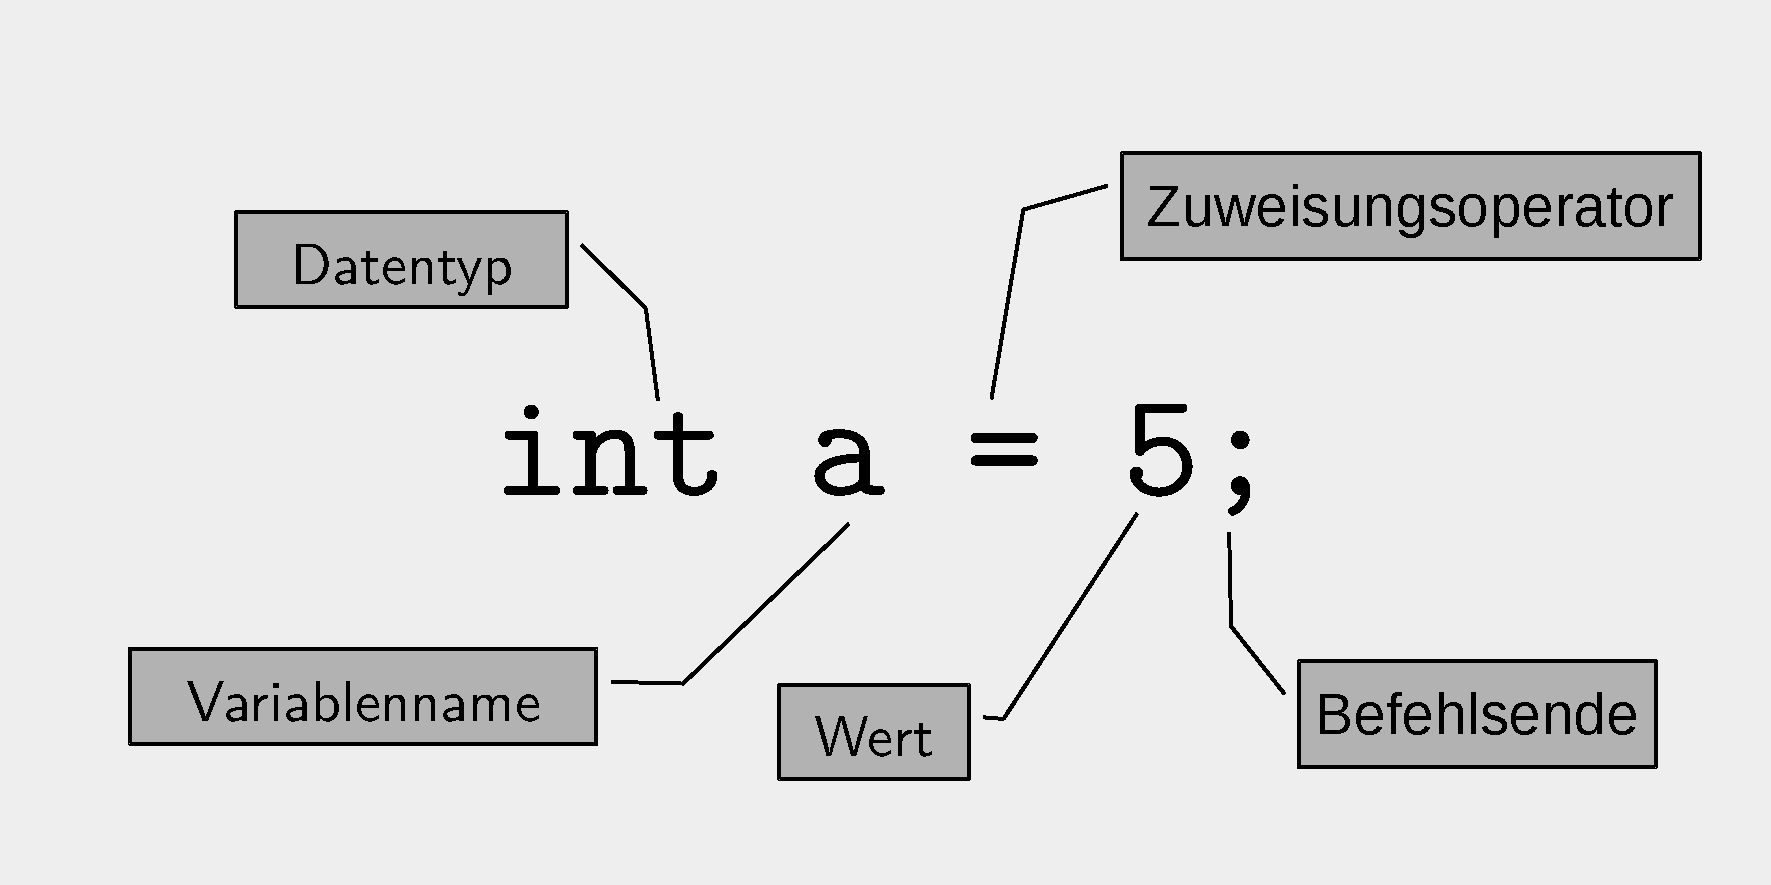
\includegraphics[width=\linewidth]{Bilder/OPL-Anweisung}
 \end{figure}
\end{frame}

\shorthandoff{"}
\subsection{Datentypen}
\begin{frame}
 \frametitle{Primitive Datentypen}
 \begin{description}
  \item[\texttt{int}] (kurz für: \glqq Integer\grqq); ein ganzzahliger Wert mit beliebigem Vorzeichen. 
  Beispielliterale: \texttt{\usebeamercolor[fg]{example text}0, 1, -2, -786}
  \item[\texttt{float}] Gleitkommazahl mit beliebigem Vorzeichen. 
  Beispielliterale: \texttt{\usebeamercolor[fg]{example text}0.0, 1.0, 3.14, -7.86}
  \item[\texttt{boolean}] eigentlich ein logischer Wahrheitswert; bei Entscheidungsvariablen eine 0-1-Variable.
  \shorthandoff{"}
  \item[\texttt{string}] eine Zeichenkette. Beispielliterale: 
  \texttt{\usebeamercolor[fg]{example text} "1", "B", "Berlin"}
  \shorthandon{"}
 \end{description}
\end{frame}


\begin{frame}
 \frametitle{Abgeleitete Datentypen}
 \begin{description}
  \item[Set] eine geordnete Menge von Elemente von (u.a) primitiven Datentypen, z.B.
  \begin{flushleft}\ttfamily\usebeamercolor[fg]{example text}
  \{string\} Standorte =\\\ \{"Ansbach", "Berlin", "Cottbus"\};
  \end{flushleft}
  \item[Array] ein über ein Set indiziertes Tupel von (u.a.) primitiven Datentypen, Sets oder anderen Arrays, z.B.
  \begin{flushleft}\ttfamily\usebeamercolor[fg]{example text}
  float Fixkosten[Standorte] =\\\ [27.4, 58.3, 30.0];
  \end{flushleft}
  Zugriff mittels Index, z.B.: \texttt{\usebeamercolor[fg]{example text}Fixkosten["Cottbus"]} \textrightarrow{} \texttt{\usebeamercolor[fg]{example text}30.0}
 \end{description}
\end{frame}
\shorthandon{"}

\begin{frame}
 \frametitle{Abgeleitete Datentypen: Mehrfache Arrays}
 \begin{itemize}
  \item Arrays können ineinander geschachtelt werden um mehrfache Indizes abzubilden, z.B.
    \begin{flushleft}\ttfamily\usebeamercolor[fg]{example text}
      float Entf[Standorte][Standorte] =\\ 
      \ [[0.0, 5.05, 4.89],\\
      \ [5.05, 0.0, 1.22],\\
      \ [4.89, 1.22, 0.0]];
    \end{flushleft}
  \item Zuordnungsregel: von links nach rechts, von außen nach innen
 \end{itemize}
\end{frame}

\subsection{Operatoren}
\begin{frame}
 \frametitle{Einfache Operatoren}
 \begin{itemize}
  \item Zuweisungsoperator \structure{\texttt{=}}
  \item Arithmetische Operatoren
  \begin{description}
   \item[\texttt{+}] Addition
   \item[\texttt{-}] Subtraktion
   \item[\texttt{*}] Multiplikation
   \item[\texttt{/}] Division (selten in linearen Modellen)
  \end{description}
  \item Vergleichsoperatoren (für lineare Modelle)
  \begin{description}
   \item[\texttt{==}] Addition
   \item[\texttt{<=}] Addition
   \item[\texttt{>=}] Addition
  \end{description}
 \end{itemize}
\end{frame}

\begin{frame}
 \frametitle{Indizierte Operatoren}
 \begin{itemize}
  \item Summenoperator
  \begin{flushleft}\Large
   {\usebeamercolor[fg]{example text}$\displaystyle\sum_{\alert{i}\in \alert{I}}\ldots$} 
   \textrightarrow{} 
   {\usebeamercolor[fg]{example text} \texttt{sum(\alert{i} in \alert{I})(\textsf{...})}}
  \end{flushleft}
  \medskip
  \item Allquantor
  \begin{flushleft}\Large
   {\usebeamercolor[fg]{example text}$\displaystyle\forall {\alert{i}\in \alert{I}}$} 
   \textrightarrow{} 
   {\usebeamercolor[fg]{example text} \texttt{forall(\alert{i} in \alert{I})}}
  \end{flushleft}
 \end{itemize}

\end{frame}


